\chapter{Security Analysis} \label{ch:security}

This chapter presents the core analytical contribution. We prove two results that
constrain the design space of covenant vaults (Sections~\ref{se:thm_griefing}
and~\ref{se:thm_inversion}), then analyze each threat model using the measured vsize
data from Chapter~\ref{ch:results}. Section~\ref{se:two_dim} synthesizes the
per-threat findings into a two-dimensional security tradeoff characterization.
Section~\ref{se:tm_matrix} presents the complete threat model matrix.
Section~\ref{se:deployment} derives fee-conditional deployment guidance.

% ======================================================================
\section{Griefing--Safety Impossibility} \label{se:thm_griefing}

The covenant literature has long discussed the tension between
keyless and key-gated recovery as a pragmatic tradeoff without
formalising the underlying dichotomy. We make that dichotomy
explicit: when recovery authorisation is expressed as a function of
cryptographic key possession, any design must choose one side, and
the choice carries inescapable consequences for both griefing
surface and key-loss risk. The proposition below captures this as
the structural root of the $(g, b)$ projection
(Lemma~\ref{lem:projection}).

\begin{definition}[Recovery Authorization] \label{def:recovery_auth}
A vault's recovery mechanism is characterized by an authorization function
$\mathcal{A}: 2^{\mathcal{K}} \rightarrow \{0,1\}$, where $\mathcal{K}$ is the
set of all cryptographic keys and $\mathcal{A}(S) = 1$ if and only if the key set
$S$ is sufficient to invoke recovery. Recovery is \emph{permissionless} if
$\mathcal{A}(\emptyset) = 1$ (no keys required) and \emph{key-gated} if
$\mathcal{A}(\emptyset) = 0$ (at least one key is required).
\end{definition}

\begin{proposition}[Griefing--Safety Incompatibility] \label{thm:griefing_safety}
Under the assumption that recovery authorization is a function of key possession
(Definition~\ref{def:recovery_auth}), no covenant vault simultaneously achieves:
\begin{enumerate}
  \item \textbf{Permissionless recovery:} $\mathcal{A}(\emptyset) = 1$
    (any party can recover without key material), and
  \item \textbf{Griefing resistance:} no unauthorized party can invoke recovery
    to deny the owner's withdrawal.
\end{enumerate}
\end{proposition}

\begin{proof}
By exhaustive case analysis over the two possible values of
$\mathcal{A}(\emptyset)$.

\emph{Case 1: $\mathcal{A}(\emptyset) = 1$ (permissionless).} Any party can
broadcast a recovery transaction without possessing key material. This maximizes
fund safety under key loss---the owner can always recover, even if all hot keys are
compromised---but any third party who can construct the recovery transaction can
force-recover the vault, denying the owner access to the normal withdrawal path.
Adding output constraints (recovery only to a pre-committed address) prevents fund
redirection but does not prevent the denial of service: the attacker can still
interrupt the owner's withdrawal by forcing recovery to the legitimate address.
CCV implements this model.

\emph{Case 2: $\mathcal{A}(\emptyset) = 0$ (key-gated).} Recovery requires a
signature from a designated key (the \texttt{recoveryauth} key in OP\_VAULT, or the
cold key in CTV, CAT+CSFS, and Simplicity). This eliminates griefing by unauthorized
parties---only the key holder can invoke recovery---but introduces key-loss risk: if
the required key is lost or destroyed, $\mathcal{A}(S) = 0$ for all available key
sets $S$, and recovery becomes permanently unavailable.

Since $\mathcal{A}(\emptyset) \in \{0, 1\}$, these two cases are exhaustive. In
Case~1, griefing resistance fails. In Case~2, permissionless recovery fails. No
vault achieves both. \qedhere
\end{proof}

\noindent
\textbf{Scope of the assumption.} The proposition assumes recovery authorization
depends solely on cryptographic key possession. It does not model non-cryptographic
gating mechanisms such as time delays on recovery, reputation systems, or
out-of-band identity verification. All five covenant designs studied in this thesis
fall within this assumption: recovery is gated by \texttt{OP\_CHECKSIG} (key-gated)
or ungated (permissionless).

The practical consequence is that vault designers must choose a point on the
griefing--safety spectrum. Table~\ref{tab:griefing_spectrum} maps each covenant to
its position.

\begin{table}[t]
\centering
\caption{Recovery model and griefing--safety tradeoff for each covenant design.}
\label{tab:griefing_spectrum}
\begin{tabular}{@{}lllll@{}}
\toprule
Covenant & Recovery model & Key required & Griefing & Key-loss risk \\
\midrule
CCV       & Keyless           & None         & Anyone can grief & None \\
OP\_VAULT & Key-gated (auth)  & recoveryauth & Auth key holder  & Auth key loss \\
CTV       & Key-gated (cold)  & Cold key     & Cold key holder  & Cold key loss \\
CAT+CSFS  & Key-gated (cold)  & Cold key     & Cold key holder  & Cold key loss \\
Simplicity & Key-gated + constrained & Cold key & Cold key holder & Cold key loss \\
\bottomrule
\end{tabular}
\end{table}

% ======================================================================
\section{Adversary Advantage and Structural Analysis} \label{se:thm_inversion}

Proposition~\ref{thm:griefing_safety} establishes a structural tradeoff
without reference to fee dynamics. To reason about how vault security
varies across designs, threat models, and fee environments uniformly,
we introduce a per-strategy loss framework. We then decompose the
covenant-vault design space into four nearly-orthogonal dimensions,
derive feature-by-feature implications for defender loss, and obtain
as a structural consequence that no proposed Bitcoin Script extension
occupies the dominant corner of the design space.

\subsection{Framework}
\label{ss:framework}

We parameterise each vault scenario by a threat model
$\mathrm{TM} \in \mathcal{T}$, a design $D \in \mathcal{D}$, a vault
value $V > 0$, a prevailing fee rate $r \geq 0$, and a boolean defender
strategy $b \in \{0, 1\}$: $b = 1$ indicates the defender batches
recovery transactions across available UTXOs; $b = 0$ indicates
single-input recovery. An adversary strategy~$\mathcal{A}$ consists of a
(possibly unbounded) sequence of on-chain transactions broadcast in
pursuit of~$\mathrm{TM}$.

\begin{definition}[Per-strategy cost and outcome] \label{def:strategy_costs}
For an adversary strategy~$\mathcal{A}$ at fee rate~$r$ we write:
$g(\mathcal{A}) \in [0, V]$ for the funds the adversary extracts to an
attacker-controlled output; $c_A(\mathcal{A}, r)$ for the on-chain fees
paid by the adversary; $c_D(\mathcal{A}, r, b)$ for the on-chain fees
paid by the defender responding optimally to~$\mathcal{A}$ under
batching strategy~$b$; and $u(\mathcal{A}) \in [0, V]$ for funds
rendered unrecoverable (dust-locked) by~$\mathcal{A}$.
\end{definition}

\begin{definition}[Defender loss and adversary advantage] \label{def:loss_adv}
Fix $(\mathrm{TM}, D, V, r, b)$ and an attacker budget $B_A$. The
\emph{worst-case defender loss} is
\[
  \mathcal{L}(\mathrm{TM}, D, V, r, b)
  \;=\; \sup_{\mathcal{A}:\, c_A(\mathcal{A}, r) \leq B_A}
    \bigl[\, g(\mathcal{A}) + u(\mathcal{A}) + c_D(\mathcal{A}, r, b) \,\bigr],
\]
taken over strategies realising~$\mathrm{TM}$ against~$D$ with
bounded attacker fee expenditure. The budget constraint formalises
the rational-adversary assumption; without it, unbounded griefing
rounds make the supremum diverge. In the per-threat analyses of
Sections~\ref{se:fee_pinning}--\ref{se:cold_key_recovery} we take
$B_A$ to be the vault value~$V$ (an attacker will not pay more in
fees than the funds at stake); the measured $\mathcal{L}$ values
are insensitive to larger choices of $B_A$.
The \emph{worst-case adversary advantage} is
$\mathrm{Adv}(\mathrm{TM}, D, V, r) =
\sup_{\mathcal{A}}[\, g(\mathcal{A}) - c_A(\mathcal{A}, r) \,]$,
which is invariant in~$b$. Design~$D_1$ is \emph{safer than} $D_2$,
written $D_1 \prec_{\mathrm{TM}, V, r, b} D_2$, iff
$\mathcal{L}(\mathrm{TM}, D_1, V, r, b) <
\mathcal{L}(\mathrm{TM}, D_2, V, r, b)$.
\end{definition}

$\mathcal{L}$ captures theft~($g > 0$), griefing~($c_D > 0$), and
dust-lockup~($u > 0$) in a single quantity comparable across threat
classes; $\mathrm{Adv}$ is positive when the attack is profit-bearing
and negative when the attacker pays for a denial-of-service outcome.
Per-threat expressions for~$\mathcal{L}$ appear in
Sections~\ref{se:fee_pinning}--\ref{se:cold_key_recovery}.

\subsection{Design-Space Decomposition}
\label{ss:design_space}

Every covenant vault design~$D$ makes a choice in four nearly-orthogonal
dimensions that together determine its on-chain attack surface.

\begin{description}
  \item[Fee model ($f$)] How covenant transactions pay miner fees. Observed
    values across the four proposed BIPs:
    \begin{itemize}
      \item $f_{\text{anchor}}$: CPFP-bumpable anchor output (CTV);
      \item $f_{\text{wallet}}$: separate fee-wallet input (OP\_VAULT);
      \item $f_{\text{inval}}$: fees deducted from input value via
        introspection (CCV);
      \item $f_{\text{acp}}$: \sighash{SINGLE}$|$\texttt{ANYONECANPAY}
        permits external fee inputs (CAT+CSFS).
    \end{itemize}
  \item[Amount flexibility ($a$)] Whether a single trigger can spend less
    than the vault's full value. $a_{\text{atomic}}$: the entire vault
    must unvault in one trigger. $a_{\text{partial}}$: trigger-and-revault
    splits input value across two outputs.
  \item[Recovery gating ($g$)] Who may invoke the recovery path.
    $g_{\text{keyless}}$: any party (CCV). $g_{\text{key}}$: an authorised
    key is required (cold key in CTV, CAT+CSFS; recoveryauth key in
    OP\_VAULT).
  \item[Recovery binding ($b$)] Whether the recovery output is
    script-constrained. $b_{\text{bound}}$: destination fixed at vault
    creation (CTV template hash; OP\_VAULT Taproot-tweak; Simplicity
    \texttt{jet::outputs\_hash()}). $b_{\text{unbound}}$: recovery leaf
    is bare \texttt{OP\_CHECKSIG} and admits any destination (CAT+CSFS
    cold leaf).
\end{description}

We write $D = (f, a, g, b)$. Two structural dependencies hold among the
dimensions: $f = f_{\text{acp}}$ forces $a = a_{\text{atomic}}$ because
\sighash{SINGLE} commits to exactly one output, which forbids the
two-output \texttt{trigger\_and\_revault} pattern;
$a = a_{\text{partial}}$ requires $f \in \{f_{\text{wallet}},
f_{\text{inval}}\}$ because per-output introspection is needed to deduct
the withdrawal amount while preserving the remainder.

\subsection{Feature--Vulnerability Implications}
\label{ss:feature_vuln}

Each feature choice deterministically opens or closes a vulnerability
surface. The implications below are consequences of the feature's
script semantics, not empirical observations about specific BIPs.

\begin{lemma}\label{lem:anchor_pinning}
Under Bitcoin Core 28.x default relay policy (25-descendant mempool
cluster limit, 3~sat/vB dust relay rate, 3{,}300-sat anchor output
size in the reference CTV implementation), $f = f_{\text{anchor}}$
implies the existence of a TM1 fee-pinning attack strategy with
$\mathcal{L}(\mathrm{TM1}) = V$. Under TRUC/v3 relay~\cite{CoreRelay}
or a future cluster-mempool policy with single-descendant opt-in,
the surface closes, and the lemma's premise no longer entails the
vulnerability. The constants are relay-policy parameters of the
Bitcoin Core reference software, not constants in BIP-119 itself.
\end{lemma}

\begin{lemma}\label{lem:revault_exhaust}
$a = a_{\text{partial}}$ implies the existence of a class-\classscale{}
per-UTXO recovery-cost scaling strategy with $\mathcal{L}(\mathrm{TM4}) > 0$ for
all $r > r^\dagger_{\mathrm{TM4}}(V, D, b)$.
Conversely, $a = a_{\text{atomic}}$ implies $\mathcal{L}(\mathrm{TM4}) = 0$
for every $r$.
\end{lemma}

\paragraph{Protocol level vs.\ user parameters.}
The \emph{existence} of a finite threshold
$r^\dagger_{\mathrm{TM4}}(V, D, b)$ is a protocol-level consequence
of Lemma~\ref{lem:revault_exhaust}: the dust-threshold attack is
definable whenever $a = a_{\text{partial}}$ holds, independent of
implementation. The numeric \emph{value} of $r^\dagger$ depends on
three parameters, none of them implementation artifacts:
$V$ is the vault value (chosen by the user at creation),
$N_{\text{budget}}$ is the defender's block budget (chosen by the
watchtower operator), and $\text{vsize}_{\text{rec}}$ is determined
by the BIP specification (script semantics fix the minimum witness
program size; signature scheme fixes witness overhead; transaction
format fixes serialisation overhead). Spec-minimal implementations
produce the same $\text{vsize}_{\text{rec}}$ up to small encoding
choices (Taproot control-block variants, nonce formats); our
measurements on the upstream reference implementations differ by
less than 5\vB{} from spec-minimal estimates. Readers reproducing
the numeric $r^\dagger$ for different vault values or defender
budgets may scale our measured values linearly without re-running
the regtest harness.

\begin{lemma}\label{lem:keyless_grief}
$g = g_{\text{keyless}}$ implies a third party can force
$\mathcal{L}(\mathrm{TM2}) > 0$ with attacker cost
$\gamma \cdot c_D$ for griefing ratio $\gamma < 1$
(Proposition~\ref{thm:griefing_safety}). $g = g_{\text{key}}$ restricts
the attacker to the designated key holder.
\end{lemma}

\begin{lemma}\label{lem:unbound_theft}
$b = b_{\text{unbound}}$ implies $\mathcal{L}(\mathrm{TM11}) = V$.
$b = b_{\text{bound}}$ implies $\mathcal{L}(\mathrm{TM11}) = 0$.
\end{lemma}

\begin{proof}[Proofs]
Each claim is direct from the feature's semantics.
Lemma~\ref{lem:anchor_pinning}: descendant-chain pinning requires an
externally-spendable output under the same ancestor-descendant mempool
cluster as the unvault transaction; $f_{\text{anchor}}$ is the only
choice producing such an output. Lemma~\ref{lem:revault_exhaust}:
\texttt{trigger\_and\_revault} is the mechanism by which the splitting
attack decreases UTXO values below the dust threshold; it is defined
only under $a = a_{\text{partial}}$. Lemma~\ref{lem:keyless_grief}:
restatement of the forward direction of
Proposition~\ref{thm:griefing_safety} under fee-rate parameterisation.
Lemma~\ref{lem:unbound_theft}: $b_{\text{unbound}}$ is precisely the
condition ``recovery output is attacker-chooseable,'' which is the
content of TM11. \qed
\end{proof}

\subsection{Structural Consequence}
\label{ss:struct_consequence}

Define the design point
\[
  D^\star \;=\; (f_{\neq\text{anchor}},\;
    a_{\text{atomic}},\; g_{\text{key}},\; b_{\text{bound}}).
\]
By Lemmas~\ref{lem:anchor_pinning}--\ref{lem:unbound_theft}, $D^\star$
has $\mathcal{L}(\mathrm{TM}_k) = 0$ for every
$\mathrm{TM}_k \in \{\mathrm{TM1}, \mathrm{TM2}, \mathrm{TM4},
\mathrm{TM11}\}$. Table~\ref{tab:design_space} locates each proposed
BIP in the $(f, a, g, b)$ lattice together with its Hamming distance
to $D^\star$.

\begin{table}[t]
\centering
\caption{The four proposed Bitcoin Script extensions located in the
$(f, a, g, b)$ design space. The column ``dist.'' gives Hamming
distance to the dominant corner
$D^\star = (f_{\neq\text{anchor}}, a_{\text{atomic}}, g_{\text{key}},
b_{\text{bound}})$.}
\label{tab:design_space}
\begin{tabular}{@{}lccccc@{}}
\toprule
Design     & $f$                 & $a$                 & $g$                    & $b$                  & dist.\ \\
\midrule
CTV        & $f_{\text{anchor}}$ & $a_{\text{atomic}}$ & $g_{\text{key}}$       & $b_{\text{bound}}$   & 1 \\
CCV        & $f_{\text{inval}}$  & $a_{\text{partial}}$ & $g_{\text{keyless}}$ & $b_{\text{bound}}$   & 2 \\
OP\_VAULT  & $f_{\text{wallet}}$ & $a_{\text{partial}}$ & $g_{\text{key}}$     & $b_{\text{bound}}$   & 1 \\
CAT+CSFS   & $f_{\text{acp}}$    & $a_{\text{atomic}}$ & $g_{\text{key}}$       & $b_{\text{unbound}}$ & 1 \\
$D^\star$  & $\neq f_{\text{anchor}}$ & $a_{\text{atomic}}$ & $g_{\text{key}}$  & $b_{\text{bound}}$   & --- \\
\bottomrule
\end{tabular}
\end{table}

\begin{proposition}\label{thm:fee_inversion}
No proposed Bitcoin Script extension occupies $D^\star$. Each of CTV,
CCV, OP\_VAULT, and CAT+CSFS differs from $D^\star$ in at least one
dimension, and that difference directly entails
$\mathcal{L}(\mathrm{TM}_k) > 0$ for the threat
$\mathrm{TM}_k \in \{\mathrm{TM1}, \mathrm{TM2}, \mathrm{TM4},
\mathrm{TM11}\}$ corresponding to the distinguishing dimension via
Lemmas~\ref{lem:anchor_pinning}--\ref{lem:unbound_theft}.
\end{proposition}

\begin{proof}
Read Table~\ref{tab:design_space} against the lemmas. CTV differs in
$f$ ($f_{\text{anchor}}$ rather than $f_{\neq\text{anchor}}$), so by
Lemma~\ref{lem:anchor_pinning} $\mathcal{L}(\mathrm{TM1}) = V > 0$.
CCV differs in $a$ and $g$, so by
Lemmas~\ref{lem:revault_exhaust} and~\ref{lem:keyless_grief} both
$\mathcal{L}(\mathrm{TM4}) > 0$ (at sufficiently high $r$) and
$\mathcal{L}(\mathrm{TM2}) > 0$. OP\_VAULT differs in $a$, so
$\mathcal{L}(\mathrm{TM4}) > 0$ at high $r$. CAT+CSFS differs in $b$,
so $\mathcal{L}(\mathrm{TM11}) = V$. No proposal matches all four
coordinates of $D^\star$. \qed
\end{proof}

\begin{corollary}\label{cor:open_corner}
The design point $D^\star$ is unoccupied by the current BIP corpus. A
specification adopting $(f_{\neq\text{anchor}}, a_{\text{atomic}},
g_{\text{key}}, b_{\text{bound}})$ would achieve $\mathcal{L} = 0$
simultaneously against $\{\mathrm{TM1}, \mathrm{TM2}, \mathrm{TM4},
\mathrm{TM11}\}$.
\end{corollary}

This corollary identifies a concrete direction for future covenant
proposals. Two current proposals are one dimension away: CTV (by
replacing its anchor-based fee model with a non-anchor alternative,
which TRUC deployment approximates) and CAT+CSFS (by replacing its
bare cold-key recovery leaf with an output-bound recovery path, as
sketched by Poelstra~\cite{Poe21} through recursive staging).
TM3 (trigger key theft) is universal across the four proposals and is
not addressed by the $(f, a, g, b)$ decomposition; we discuss its
incorporation in a future framework (Chapter~\ref{ch:discussion}).

\subsection{Relationship to Proposition~\ref{thm:griefing_safety}}
\label{ss:relation_griefing}

Proposition~\ref{thm:griefing_safety} is the projection of the
design-space analysis onto the $(g, b)$ sublattice.
Lemma~\ref{lem:keyless_grief} is its formal restatement under the
present framework. Where Proposition~\ref{thm:griefing_safety}
captures a single structural tradeoff (recovery-gating against
griefing), the 4-dimensional decomposition captures the full set of
tradeoffs visible at the covenant Script layer. Future BIPs can be
localised in the lattice by reading their specification; their
vulnerability profile follows from
Lemmas~\ref{lem:anchor_pinning}--\ref{lem:unbound_theft} without
further measurement.

\subsection{Fee-Rate Sensitivity of TM4}
\label{ss:tm4_sensitivity}

The TM4 counterexample in the proof of Proposition~\ref{thm:fee_inversion}
is the only one whose existence depends on the fee rate. We
characterise the dependence because the threshold~$r^\dagger$ is the
most operationally consequential parameter for practitioners deploying
CCV or OP\_VAULT vaults. For the remainder of this subsection, fix
$\mathrm{TM} = \mathrm{TM4}$ and consider the attacker classes CTV
(immune) versus CCV and OP\_VAULT (vulnerable).

\emph{Fee pinning cost.} The fee pinning attack against CTV requires constructing
25 descendant transactions off the unvault anchor output. The attack cost is:

\begin{equation} \label{eq:pin_cost}
C_{\text{pin}} = 25 \times (\text{dustRelay} + 1) \times \text{vsize}_{\text{desc}}
  + \text{anchor\_sats}
\end{equation}

\noindent
where $\text{dustRelay} = 3$~sat/vB is the dust relay fee, $\text{vsize}_{\text{desc}}
\approx 110$\vB{} per descendant, and $\text{anchor\_sats} = 3{,}300$. This yields
$C_{\text{pin}} \approx 14{,}300$~sats, independent of the prevailing fee rate~$r$.
Fee pinning cost is \emph{fee-invariant}: the attacker pays dust-rate fees regardless
of the fee environment.

\emph{Watchtower exhaustion cost.} The per-UTXO recovery-cost scaling attack against CCV or
OP\_VAULT requires the attacker to repeatedly split the vault into smaller UTXOs via
\texttt{trigger\_and\_revault}. Each split costs the attacker
$\text{vsize}_{\text{trigger}} \times r$ in fees. The number of splits needed to
exhaust the vault to dust-unrecoverable levels. A UTXO becomes \emph{dust} (uneconomical
to recover) when its value falls below the recovery transaction fee
$\text{vsize}_{\text{recover}} \times r$. The number of splits needed to reduce every
fragment below this dust threshold is:

\begin{equation} \label{eq:splits}
N_{\text{dust}}(r) = \left\lfloor \frac{V}{\text{vsize}_{\text{recover}} \times r}
  \right\rfloor
\end{equation}

\noindent
where $V$ is the vault value in sats, $\text{vsize}_{\text{recover}}$ is the
recovery transaction size, and $r$ is the fee rate. $N_{\text{dust}}$ gives the
number of fragments at which each fragment's value equals the cost to recover it.
As $r$ increases, the dust threshold rises, so fewer splits are needed to make
individual UTXOs unrecoverable. The total
attacker cost is:

\begin{equation} \label{eq:exhaust_cost}
C_{\text{exhaust}}(r) = N_{\text{splits}}(r) \times \text{vsize}_{\text{trigger}}
  \times r
\end{equation}

\paragraph{Dust-threshold fee rate.}
The defender-loss under TM4 is dominated by whether individual dust
UTXOs can be economically recovered. Define the single-block
feasibility threshold $r^\dagger_{\mathrm{TM4}}(V, D, b)$ as the fee
rate at which an attacker can fully exhaust a vault of value~$V$
within one block under defender batching strategy~$b$. Using measured
vsize values from Chapter~\ref{ch:results}, the unbatched thresholds
for a 0.5~BTC vault are approximately $r^\dagger(V, \mathrm{CCV}, 0)
\approx 66\satvB$ and $r^\dagger(V, \mathrm{OP\_VAULT}, 0) \approx
59\satvB$. Below these rates, the TM4 attack is infeasible; above
them, $\mathcal{L}(\mathrm{TM4})$ approaches $V$ and the design
becomes vulnerable. The CTV fee-pinning cost of
Equation~\ref{eq:pin_cost} is negligible relative to~$V$ for any
practical vault size, so CTV dominates CCV and OP\_VAULT under TM4 at
any~$r$, consistent with the TM4 counterexample in the proof of
Proposition~\ref{thm:fee_inversion}.

\paragraph{Scope of the threshold analysis.}
Equations~\ref{eq:splits}--\ref{eq:exhaust_cost} assume single-input
recovery by the defender ($b = 0$). BIP-345 and BIP-443 both permit
batched recovery in which $N$ Unvaulting UTXOs are spent into a
single recovery transaction, amortising fixed overhead across
inputs. Section~\ref{ss:batched_defender} revisits the threshold
under the batched strategy ($b = 1$); the batched thresholds are
approximately $1.8\times$~(CCV) and $2.7\times$~(OP\_VAULT) the
unbatched values and reverse the two designs' relative vulnerability
under TM4.

\paragraph{Sensitivity to vault value.}
The crossover fee rate $r^*$ depends on the vault value $V$. From
Equation~\ref{eq:splits}, the number of blocks needed for per-UTXO recovery-cost scaling is:

\begin{equation} \label{eq:blocks_exhaust}
B(r, V) = \frac{V}{\text{vsize}_{\text{recover}} \times r \times S}
\end{equation}

\noindent
where $S$ is the splits per block (6{,}172 for CCV). Setting $B = B_{\max}$
(a practical feasibility threshold) and solving for $r$:

\begin{equation} \label{eq:r_star}
r^*(V) = \frac{V}{\text{vsize}_{\text{recover}} \times B_{\max} \times S}
\end{equation}

\noindent
Table~\ref{tab:r_star_sensitivity} shows $r^*$ across vault values at two
thresholds: $B_{\max} = 10$ blocks (${\sim}100$ minutes, a sustained but feasible
attack) and $B_{\max} = 1$ block (single-block exhaustion).

\paragraph{Defender-budget interpretation.}
Equation~\ref{eq:r_star} parameterises $r^*$ by the attacker's
block-budget $B_{\max}$. The equivalent defender-side parameter is
$N_{\mathrm{budget}} = B_{\max} \cdot S_{\mathrm{recover}}$, the
number of Unvaulting UTXOs the watchtower can recover within
$B_{\max}$ blocks at recovery throughput $S_{\mathrm{recover}}$
(blocks-worth of recoveries per block, $S_{\mathrm{recover}} =
\lfloor 4{,}000{,}000 / (4 \cdot \text{vsize}_{\text{recover}}) \rfloor$
under single-input recovery, larger under batching per
Section~\ref{ss:batched_defender}). The threshold $r^\dagger$
scales linearly in $N_{\mathrm{budget}}$: doubling the defender's
recovery capacity doubles the fee rate at which the attack becomes
feasible.

\begin{table}[t]
\centering
\caption{Crossover fee rate $r^*$ as a function of vault value $V$ for CCV.
Below $r^*$, per-UTXO recovery-cost scaling requires more than $B_{\max}$ blocks
(infeasible). Above $r^*$, exhaustion completes within $B_{\max}$ blocks.}
\label{tab:r_star_sensitivity}
\begin{tabular}{@{}rrr@{}}
\toprule
Vault value $V$ & $r^*$ at $B_{\max} = 10$ & $r^*$ at $B_{\max} = 1$ \\
(BTC)           & (sat/vB)                  & (sat/vB) \\
\midrule
0.01 &   0.1 &    1.3 \\
0.10 &   1.3 &   13.3 \\
0.50 &   6.6 &   66.4 \\
1.00 &  13.3 &  132.8 \\
5.00 &  66.4 &  664.0 \\
10.00 & 132.8 & 1{,}328 \\
\bottomrule
\end{tabular}
\end{table}

The crossover scales linearly with vault value: larger vaults require higher fee
rates before exhaustion becomes feasible (more splits needed). A 0.1~BTC vault is
vulnerable to single-block exhaustion at 13\satvB{}---well within normal fee ranges.
A 5~BTC vault requires 664\satvB{} for single-block exhaustion, which has occurred
only during extreme congestion events. This parameterization gives practitioners a
direct tool: given their vault value and risk tolerance, they can determine the fee
regime where CCV/OP\_VAULT's watchtower exposure exceeds CTV's fee pinning risk.

Figure~\ref{fig:fee_inversion} illustrates the crossover for a 0.5~BTC vault.
The fee pinning cost curve is flat; the per-UTXO recovery-cost scaling curve decreases
hyperbolically as fees rise.

\begin{figure}[t]
\centering
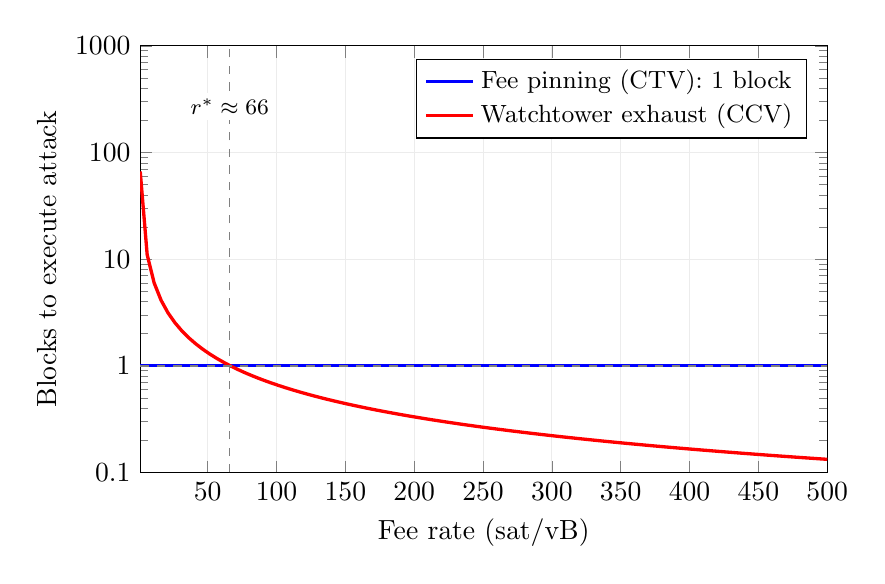
\begin{tikzpicture}
\begin{axis}[
  width=0.85\textwidth,
  height=7cm,
  xlabel={Fee rate (sat/vB)},
  ylabel={Blocks to execute attack},
  xmin=1, xmax=500,
  ymode=log,
  ymin=0.1, ymax=1000,
  legend pos=north east,
  legend style={font=\small},
  grid=major,
  grid style={gray!15},
  ytick={0.1,1,10,100,1000},
  yticklabels={0.1,1,10,100,\num{1000}},
]
% Fee pinning — always 1 block (broadcast 25 descendants, wait for CSV expiry)
\addplot[very thick, blue, domain=1:500] {1};
\addlegendentry{Fee pinning (CTV): 1 block}

% Watchtower exhaustion — CCV
% splits = V / (recover * r) = 50000000 / (122 * r)
% blocks = splits / splits_per_block = 50000000 / (122 * r * 6172)
\addplot[very thick, red, domain=1:500, samples=100]
  {50000000 / (122 * x * 6172)};
\addlegendentry{Watchtower exhaust (CCV)}

% Feasibility threshold — below 1 block = executable in single block
\draw[dashed, gray, thick] (axis cs:1,1) -- (axis cs:500,1);

% Crossover annotation — where CCV drops below ~10 blocks (practical)
\draw[dashed, gray] (axis cs:66,0.1) -- (axis cs:66,1000);
\node[font=\footnotesize, fill=white, inner sep=2pt, anchor=south]
  at (axis cs:66,200) {$r^* \approx 66$};

\end{axis}
\end{tikzpicture}
\caption{Fee-dependent security inversion. CTV fee pinning (blue) executes in
one block regardless of fee rate. CCV per-UTXO recovery-cost scaling (red) requires
progressively fewer blocks as fees rise, because each split creates a larger
dust threshold. Below ${\sim}50$~sat/vB, exhaustion requires hundreds of blocks
(infeasible). Above $r^* \approx 66$~sat/vB, exhaustion completes within a few
blocks, making it practical. The crossover defines where the safety ranking inverts.}
\label{fig:fee_inversion}
\end{figure}

% ======================================================================
\section{Class \classfee{}: Fee-Channel Pinning (TM1)} \label{se:fee_pinning}

Fee pinning exploits CTV's anchor-based fee management. The unvault transaction
includes an anchor output at \texttt{vout=1} (3{,}300~sats) to enable CPFP fee
bumping. An attacker with the hot key broadcasts the unvault, then immediately
constructs 25 low-fee descendant transactions spending the anchor output. Bitcoin
Core's mempool policy limits descendant chains to 25 transactions; once the limit
is reached, the watchtower's CPFP recovery transaction is rejected because it would
exceed the descendant count.

\begin{figure}[t]
\centering
\resizebox{0.95\textwidth}{!}{%
\begin{tikzpicture}[
  tx/.style={rectangle, draw, rounded corners=2pt, minimum width=1.8cm,
             minimum height=0.75cm, align=center, font=\scriptsize,
             fill=blue!5, draw=blue!60!black, thick},
  descendant/.style={rectangle, draw, minimum width=0.55cm, minimum height=0.55cm,
                     font=\tiny, fill=orange!20, draw=orange!60!black},
  wtx/.style={rectangle, draw, rounded corners=2pt, minimum width=1.8cm,
              minimum height=0.75cm, align=center, font=\scriptsize,
              fill=green!10, draw=green!60!black, thick},
  rej/.style={rectangle, draw, rounded corners=2pt, minimum width=2.2cm,
              minimum height=0.75cm, align=center, font=\scriptsize,
              fill=red!10, draw=red!60!black, thick},
  phase/.style={font=\scriptsize\bfseries, align=center, text=gray!60!black},
  note/.style={font=\scriptsize, align=center, text=gray!70!black},
  edge/.style={draw, ->, >=stealth, thick},
  lane/.style={rectangle, rounded corners=4pt, thick, dash pattern=on 3pt off 2pt},
]
  % ===== Top lane: attacker =====
  \node[lane, fill=red!2, draw=red!40!black, minimum width=14.5cm,
        minimum height=2.4cm] (alane) at (6.5, 2.0) {};
  \node[font=\small\bfseries, text=red!70!black, anchor=west]
       at ($(alane.north west)+(0.2,-0.3)$) {Attacker};

  % Phase 1
  \node[phase] at (1.4, 3.3) {\textcircled{\scriptsize 1} Broadcast unvault};
  \node[tx] (unvault) at (1.4, 1.9) {Unvault TX};

  % Phase 2: descendant chain
  \node[phase] at (6.3, 3.3) {\textcircled{\scriptsize 2} Chain 25 dust-fee descendants};
  \node[descendant] (d1) at (4.2, 1.9) {1};
  \node[descendant, right=0.08cm of d1] (d2) {2};
  \node[descendant, right=0.08cm of d2] (d3) {3};
  \node[font=\tiny, right=0.08cm of d3] (dots) {$\cdots$};
  \node[descendant, right=0.08cm of dots] (d24) {24};
  \node[descendant, right=0.08cm of d24, fill=red!25, draw=red!70!black] (d25) {\textbf{25}};
  \draw[->, thin, gray] (d1) -- (d2);
  \draw[->, thin, gray] (d2) -- (d3);
  \draw[->, thin, gray] (d24) -- (d25);
  \draw[->, thin, orange!70!black] (unvault.east) -- (d1.west);

  % Phase 4: withdrawal confirms (same lane)
  \node[phase] at (11.7, 3.3) {\textcircled{\scriptsize 4} CSV expires: theft};
  \node[tx, fill=red!15, draw=red!70!black] (theft) at (11.7, 1.9)
       {Withdraw TX\\ \scriptsize confirms};

  % ===== Bottom lane: watchtower =====
  \node[lane, fill=blue!2, draw=blue!40!black, minimum width=14.5cm,
        minimum height=2.0cm] (wlane) at (6.5, -0.6) {};
  \node[font=\small\bfseries, text=blue!70!black, anchor=west]
       at ($(wlane.north west)+(0.2,-0.3)$) {Watchtower};

  % Phase 3: CPFP rejected
  \node[phase] at (6.3, 0.5) {\textcircled{\scriptsize 3} CPFP blocked by mempool policy};
  \node[wtx] (cpfp) at (4.4, -0.9) {CPFP tx};
  \node[rej] (rejected) at (8.3, -0.9)
       {REJECTED\\ \scriptsize 25-descendant cap};
  \draw[edge, red!60!black, dashed] (cpfp.east) -- (rejected.west);
  \node[font=\Large, text=red!80!black] at (6.35, -0.9) {$\times$};

  % Monitor arrow (attacker -> watchtower)
  \draw[edge, dashed, blue!60!black] (unvault.south) -- ++(0,-0.6) -| (cpfp.north)
        node[pos=0.75, left, note] {monitor};

  % Theft consequence arrow (straight, same lane)
  \draw[edge, red!70!black, thick] (d25.east) -- (theft.west)
        node[midway, above=1pt, note, text=red!70!black] {pin holds $\Rightarrow$ theft};

  % ===== Timeline axis =====
  \draw[->, thick, gray!50] (-0.5, -2.3) -- (13.5, -2.3);
  \node[note, below=0.05cm of {(-0.2,-2.3)}] {$t = 0$};
  \node[note, below=0.05cm of {(11.7,-2.3)}] {$t = \text{CSV}$};

  % Annotation box
  \node[align=center, font=\scriptsize, fill=yellow!10, draw=gray!50,
        rounded corners=1pt, inner sep=3pt, text width=7.5cm]
       at (6.5, -3.2)
       {\textbf{Bitcoin Core policy:} max 25 descendants per ancestor.
        Once reached, any new CPFP would exceed the cap and is rejected.};

\end{tikzpicture}}
\caption{Fee pinning attack against CTV (\textbf{TM1}).
\textcircled{\scriptsize 1}~Attacker broadcasts the unvault, starting the CSV
window. \textcircled{\scriptsize 2}~Attacker chains 25 dust-rate descendants off
the anchor output, filling the mempool descendant limit.
\textcircled{\scriptsize 3}~The watchtower's CPFP recovery is rejected by mempool
policy (adding it would exceed the 25-descendant cap).
\textcircled{\scriptsize 4}~When CSV expires, the attacker's pre-committed
withdrawal confirms.}
\label{fig:fee_pinning}
\end{figure}

The attack cost function (Equation~\ref{eq:pin_cost}) evaluates to approximately
14{,}300~sats at dust-rate fees, regardless of the prevailing fee environment. At a
vault value of 0.5~BTC (50{,}000{,}000~sats), the attack costs 0.03\% of the vault
value---well below any economic rationality threshold.

CCV, OP\_VAULT, and CAT+CSFS are immune to this specific attack. CCV and OP\_VAULT
do not use anchor outputs (fees are paid via separate mechanisms). CAT+CSFS uses
\texttt{SIGHASH\_SINGLE|ANYONECANPAY}, which allows external fee inputs without
an anchor output.

\paragraph{Timing assumption.}
The attack requires the attacker to broadcast all 25 descendant transactions and
have them accepted into mempools \emph{before} the watchtower broadcasts its CPFP
recovery transaction. On mainnet, a well-configured watchtower would have its CPFP
transaction pre-constructed and ready to broadcast immediately upon detecting the
unvault. The attack therefore depends on a propagation race: the attacker must fill
the descendant chain across a sufficient fraction of the network's mempools before
the watchtower's single CPFP transaction propagates. Our regtest experiment
(Chapter~\ref{ch:results}) demonstrates that the descendant chain construction is
structurally valid---the 25-transaction chain is accepted and the CPFP is
rejected---but cannot test the propagation race, because regtest has a single
mempool with no network latency. The practical feasibility of this attack on mainnet
depends on the relative propagation speeds of the attacker's 25~transactions versus
the watchtower's single transaction, which is a network-layer question outside the
scope of this work (see Section~\ref{se:limitations} for further discussion).

TRUC/v3 transactions (merged in Bitcoin Core 28.0) limit descendant chains to a
single transaction. If CTV vault transactions opt into TRUC, the 25-descendant
pinning vector is eliminated at the relay policy level, potentially changing the
crossover result of Proposition~\ref{thm:fee_inversion}.

% ======================================================================
\section{Class \classscale{}: Per-UTXO Recovery-Cost Scaling (TM4)} \label{se:watchtower_exhaustion}

CCV and OP\_VAULT support partial withdrawals via \texttt{trigger\_and\_revault},
which splits the vault into a withdrawal portion and a re-locked remainder. An
attacker with the trigger key can repeatedly invoke this operation, splitting the
vault into progressively smaller UTXOs. When individual UTXOs become small enough
that the recovery transaction fee exceeds the UTXO value, those funds are
effectively lost---the watchtower cannot economically justify recovering them.

\begin{figure}[t]
\centering
\resizebox{0.95\textwidth}{!}{%
\begin{tikzpicture}[
  vault/.style={rectangle, draw, rounded corners=2pt, align=center,
                font=\scriptsize, fill=blue!15, draw=blue!70!black, thick},
  mid/.style={rectangle, draw, rounded corners=1pt, align=center,
              font=\scriptsize, fill=blue!10, draw=blue!60!black},
  small/.style={rectangle, draw, rounded corners=1pt, align=center,
                font=\tiny, fill=blue!6, draw=blue!60!black,
                minimum width=0.9cm, minimum height=0.5cm},
  dust/.style={rectangle, draw, rounded corners=1pt, align=center,
               font=\tiny, fill=red!20, draw=red!70!black,
               minimum width=0.8cm, minimum height=0.4cm},
  phase/.style={font=\scriptsize\bfseries, text=gray!60!black, align=center},
  note/.style={font=\scriptsize, align=center, text=gray!70!black},
  edge/.style={draw, ->, >=stealth, thick},
]
  % Phase headers
  \node[phase] at (0, 3.2)   {Initial};
  \node[phase] at (4.0, 3.2) {Round 1};
  \node[phase] at (8.0, 3.2) {Round $k$};
  \node[phase] at (12.0, 3.2) {Below dust};

  % Initial vault
  \node[vault, minimum width=2.6cm, minimum height=1.3cm] (v0) at (0, 1.5)
       {Vault $V$\\ 50M sats};

  % Round 1: two halves
  \node[mid, minimum width=2.2cm, minimum height=0.8cm] (v1a) at (4.0, 2.2)
       {revault 25M};
  \node[mid, minimum width=2.2cm, minimum height=0.8cm] (v1b) at (4.0, 0.8)
       {revault 25M};
  \draw[edge] (v0.east) -- ++(0.3,0) |- (v1a.west);
  \draw[edge] (v0.east) -- ++(0.3,0) |- (v1b.west);

  % Round k: many small UTXOs (shown as grid)
  \node[small] (s1) at (7.4, 2.4) {500k};
  \node[small, right=0.08cm of s1] (s2) {500k};
  \node[small, right=0.08cm of s2] (s3) {500k};
  \node[small] (s4) at (7.4, 1.7) {500k};
  \node[small, right=0.08cm of s4] (s5) {500k};
  \node[small, right=0.08cm of s5] (s6) {500k};
  \node[small] (s7) at (7.4, 1.0) {500k};
  \node[small, right=0.08cm of s7] (s8) {500k};
  \node[font=\tiny, right=0.08cm of s8] {$\cdots$};
  \draw[->, thin, gray] (v1a.east) -- ++(0.3,0) |- (s2.west);
  \draw[->, thin, gray] (v1b.east) -- ++(0.3,0) |- (s7.west);

  % Below dust
  \node[dust] (d1) at (11.5, 2.4) {5k};
  \node[dust, right=0.08cm of d1] (d2) {5k};
  \node[dust, right=0.08cm of d2] (d3) {5k};
  \node[dust] (d4) at (11.5, 1.7) {5k};
  \node[dust, right=0.08cm of d4] (d5) {5k};
  \node[dust, right=0.08cm of d5] (d6) {5k};
  \node[dust] (d7) at (11.5, 1.0) {5k};
  \node[dust, right=0.08cm of d7] (d8) {5k};
  \node[font=\tiny, right=0.08cm of d8] {$\cdots$};
  \draw[->, thin, red!60!black, dashed] (s8.east) -- ++(0.35,0) |- (d5.west);

  % Dust threshold bar (ABOVE the dust row, not cutting through others)
  \draw[red!70!black, thick, dashed] (10.3, 3.0) -- (10.3, 0.4);
  \node[font=\scriptsize\bfseries, text=red!70!black, rotate=90, anchor=south]
        at (10.15, 1.7) {dust threshold};

  % Bottom: formula and explanation
  \node[align=center, font=\scriptsize, fill=yellow!10, draw=gray!50,
        rounded corners=2pt, inner sep=5pt, text width=5cm] at (3.0, -0.6)
       {\textbf{Splits to exhaust vault:}\\[2pt]
        $N_{\text{dust}}(r) =
         \left\lfloor \dfrac{V}{\text{vsize}_{\text{rec}} \times r} \right\rfloor$};

  \node[align=left, font=\scriptsize, fill=red!5, draw=red!50,
        rounded corners=2pt, inner sep=5pt, text width=5.8cm]
        at (9.3, -0.6)
       {\textbf{Recovery fee per UTXO:} $122\vB \times r$ sats\\[1pt]
        At high $r$, many UTXOs fall below the dust threshold:
        the watchtower cannot economically justify recovery,
        and those funds are effectively lost.};

\end{tikzpicture}}
\caption{Watchtower exhaustion via \texttt{trigger\_and\_revault} (\textbf{TM4}).
The attacker (holding the trigger key) repeatedly splits the vault into smaller
UTXOs. As UTXOs shrink, the per-recovery fee ($\text{vsize}_{\text{rec}} \times r$)
consumes an increasing fraction of each UTXO's value. Once a UTXO's value falls
below $\text{vsize}_{\text{rec}} \times r$, the watchtower cannot economically
justify recovery---those funds are effectively lost.}
\label{fig:watchtower_exhaustion}
\end{figure}

Using the measured transaction sizes from Chapter~\ref{ch:results}, we compute the
splitting capacity per block. Each \texttt{trigger\_and\_revault} transaction weighs
approximately 648~WU for CCV and 1{,}168~WU for OP\_VAULT. The maximum block weight
is 4{,}000{,}000~WU, yielding:

\begin{align}
\text{CCV splits/block}      &\approx \frac{4{,}000{,}000}{648} \approx 6{,}172 \\
\text{OP\_VAULT splits/block} &\approx \frac{4{,}000{,}000}{1{,}168} \approx 3{,}427
\end{align}

Harding~\cite{Har24} estimated approximately 3{,}000 splits per block based on
assumed OP\_VAULT-sized transactions. Our measurement confirms this for OP\_VAULT
(3{,}427, within 14\% of the estimate) but reveals that CCV achieves approximately
80\% more splits per block due to its smaller trigger transaction (162\vB{} vs.\
292\vB{}). This correction matters because CCV (BIP-443) is the active proposal
that replaced OP\_VAULT (BIP-345): the design that Bitcoin is most likely to adopt
has a larger per-UTXO recovery-cost scaling surface than previously estimated.

The watchtower's recovery budget determines how many splits it can absorb. At
fee rate~$r$, recovering a single split costs $\text{vsize}_{\text{recover}} \times r$
sats (122$r$ for CCV, 246$r$ for OP\_VAULT). The total recovery budget needed to
defend against $N$ splits is $N \times \text{vsize}_{\text{recover}} \times r$.
For a 0.5~BTC vault at 100\satvB{}, defending against 1{,}000 splits costs
$1{,}000 \times 122 \times 100 = 12{,}200{,}000$~sats (0.122~BTC)---roughly 24\%
of the vault value.

\subsection{Batched Defender Strategy}
\label{ss:batched_defender}

The analysis above assumes single-input recovery: one transaction per
recovered Unvaulting UTXO. BIP-345's ``Batching'' section (authorized
recovery, lines 613--621) and BIP-443's default aggregation mode both
permit the defender to recover $N$ UTXOs in a single transaction, with
vsize scaling as $\alpha + \beta \cdot N$ where $\alpha$ is fixed
overhead and $\beta$ is the marginal per-input cost. We measure both
constants empirically on regtest, sweeping $N \in \{2, 5, 10, 25, 50\}$
and extracting $(\alpha, \beta)$ by linear regression:

\begin{table}[h]
\centering
\caption{Measured batched-recovery constants on regtest. The fit
$\text{vsize}(N) = \alpha + \beta \cdot N$ replaces the single-input
$\text{vsize}_{\text{recover}}$ with an amortized per-UTXO cost
$\alpha/N + \beta \to \beta$ for large $N$.}
\label{tab:batched_recovery}
\begin{tabular}{@{}lccccc@{}}
\toprule
Design     & $\alpha$ (\vB) & $\beta$ (\vB) & Unbatched $r^\dagger$ & Batched $r^\dagger$ & Factor \\
\midrule
CCV        & 54  & 68 & 66\satvB  & 119\satvB & $1.8\times$ \\
OP\_VAULT  & 154 & 92 & 59\satvB  & 159\satvB & $2.7\times$ \\
\bottomrule
\end{tabular}
\end{table}

Substituting $\beta$ for $\text{vsize}_{\text{recover}}$ in
Equation~\ref{eq:r_star} yields the batched dust-threshold
$r^\dagger_{\text{batched}}(V, D) = V / (\beta(D) \times S(D))$. For
a 0.5~BTC vault the batched thresholds rise to 119\satvB{} for CCV and
159\satvB{} for OP\_VAULT---roughly $1.8\times$ and $2.7\times$ the
unbatched values. The larger multiplier for OP\_VAULT reflects its
larger unbatched recovery transaction (246\vB{}): batching amortizes
that overhead more aggressively than CCV's already-small 122\vB{}
recovery.

\paragraph{Batching flips the TM4 ordering.}
Unbatched, CCV is safer than OP\_VAULT against per-UTXO recovery-cost scaling
($r^\dagger$ 66 vs 59). Once the defender batches, the ordering flips:
OP\_VAULT becomes safer ($r^\dagger$ 159 vs 119). The intuition is that
CCV's lead under single-input recovery comes from a smaller
$\text{vsize}_{\text{recover}}$, but under batching the relevant cost
is the marginal per-input $\beta$, which is nearly equal across the
two designs (68 vs 92\vB). OP\_VAULT's lower splits-per-block
($S = 3{,}427$ vs $6{,}172$) then dominates, yielding the higher
$r^\dagger$. The operational implication is that the
``CCV has a larger per-UTXO recovery-cost scaling surface'' conclusion of the
unbatched analysis reverses once watchtower operators adopt batched
recovery---a non-trivial finding for vault designers choosing between
BIP-443 and BIP-345.

\paragraph{Constraints on batched recovery.}
BIP-345's authorized recovery permits batching across vaults with
distinct \texttt{<recovery-sPK-hash>} values (§``Batching'' lines
618--621), allowing a single watchtower to serve multiple independent
users in one transaction. Unauthorized recovery is capped at two
outputs (lines 389--391) and thus limited to same-\texttt{recovery-sPK}
batches. BIP-443's default aggregation has no taptree-equivalence
requirement and is strictly more permissive. The attacker's
\texttt{trigger\_and\_revault} sequence is inherently serial---each
revault consumes the previous output---so the attacker does not
benefit from batching. The measured savings accrue asymmetrically to
the defender.

CTV, CAT+CSFS, and Simplicity are immune to per-UTXO recovery-cost scaling because they do
not support partial withdrawals. The entire vault balance must be unvaulted
atomically, so the watchtower needs only one recovery transaction regardless of
attack persistence.

% ======================================================================
\section{Class \classgrief{}: Permissionless Griefing (TM2)} \label{se:recovery_griefing}

Recovery griefing is a denial-of-service attack where the adversary repeatedly
invokes recovery to prevent the vault owner from completing withdrawals. The
economic asymmetry between attacker and defender costs determines the severity.

\begin{figure}[t]
\centering
\resizebox{0.9\textwidth}{!}{%
\begin{tikzpicture}[
  node distance=1.0cm,
  actor/.style={rectangle, draw, rounded corners=2pt, minimum width=3.0cm,
                minimum height=1.0cm, align=center, font=\small,
                thick},
  attacker/.style={actor, fill=red!10, draw=red!60!black},
  defender/.style={actor, fill=blue!10, draw=blue!60!black},
  action/.style={rectangle, draw, rounded corners=1pt, minimum width=2.5cm,
                 minimum height=0.6cm, align=center, font=\scriptsize,
                 fill=gray!5},
  cost/.style={font=\scriptsize, text=red!70!black, align=center},
  note/.style={font=\scriptsize, align=center, text=gray!70!black},
  edge/.style={draw, ->, >=stealth, thick},
]
  % Attacker side
  \node[attacker] (att) at (0, 0) {\textbf{Attacker}\\ (keyless in CCV)};

  % Defender side
  \node[defender] (def) at (8, 0) {\textbf{Defender}\\ (owner)};

  % Action 1: attacker invokes recovery
  \node[action, below=1.5cm of att] (act1) {Invoke recovery};
  \node[cost, below=0.05cm of act1] (c1) {122 vB};
  \draw[edge, red!60!black] (att.south) -- (act1.north);

  % Fund state 1
  \node[font=\scriptsize, align=center, fill=yellow!20, draw=gray!50,
        rounded corners=1pt, right=1.3cm of act1, inner sep=3pt, minimum height=0.7cm]
       (s1) {funds in\\ recovery addr};

  % Action 2: defender re-deposits + re-triggers
  \node[action, below=1.3cm of def] (act2) {Re-deposit\\ + re-trigger};
  \node[cost, below=0.05cm of act2, text=blue!70!black] (c2) {454 vB};
  \draw[edge, blue!60!black] (def.south) -- (act2.north);

  % Loop arrow
  \draw[edge, red!60!black, dashed] (act1.east) -- (s1.west);
  \draw[edge, blue!60!black, dashed] (s1.east) -- (act2.west);
  \draw[edge, red!70!black, thick, rounded corners=8pt]
       (act2.south) -- ++(0,-0.8) -- ++(-6.5,0) -- ++(0,2.5) -- (att.south)
       node[midway, above, note, text=red!70!black, pos=0.45] {\textbf{loop}};

  % Asymmetry indicator
  \node[align=center, font=\small, text width=5cm, fill=red!5,
        draw=red!50, rounded corners=2pt, inner sep=4pt]
       at (4, -4) {\textbf{Asymmetry:} $\gamma = \dfrac{122}{454} = 0.27$\\
                  Attacker pays $<\tfrac{1}{3}$ of defender cost};

\end{tikzpicture}}
\caption{Recovery griefing loop (\textbf{TM2}) for CCV. The attacker triggers
permissionless recovery (122\vB{}); the owner must re-deposit and re-trigger
(454\vB{}) to resume withdrawal; the attacker invokes recovery again. The
per-round cost asymmetry $\gamma = 0.27$ strongly favors the attacker.}
\label{fig:recovery_griefing}
\end{figure}

Table~\ref{tab:griefing_costs} compares the per-round costs. The griefing ratio
$\gamma = \text{vsize}_{\text{attack}} / \text{vsize}_{\text{defend}}$ measures the
cost asymmetry: $\gamma < 1$ means the attacker pays less than the defender per
round (favorable to the attacker).

\begin{equation} \label{eq:griefing_ratio}
\gamma = \frac{\text{vsize}_{\text{attack}}}{\text{vsize}_{\text{defend}}}
\end{equation}

\begin{table}[t]
\centering
\caption{Recovery griefing cost comparison. The attacker invokes recovery; the
defender re-deposits and re-triggers. $\gamma < 1$ favors the attacker.}
\label{tab:griefing_costs}
\small
\begin{tabular}{@{}llrrrl@{}}
\toprule
Covenant & Key required & Attacker & Defender & $\gamma$ & Assessment \\
         &              & (vB/round) & (vB/round) & & \\
\midrule
CCV       & None (keyless)  & 122 & 454 & 0.27 & Severe (anyone) \\
OP\_VAULT & recoveryauth    & 246 & 446 & 0.55 & Low (key needed) \\
CTV       & Hot key         & 94  & 133 & 0.71 & Moderate (reversed) \\
CAT+CSFS  & Cold key        & 125 & 343 & 0.36 & Irrelevant (TM11) \\
\bottomrule
\end{tabular}
\end{table}

CCV has the most severe griefing profile: the attack is keyless (anyone can invoke
recovery) and the cost asymmetry strongly favors the attacker ($\gamma = 0.27$).
OP\_VAULT eliminates anonymous griefing by requiring the \texttt{recoveryauth} key,
raising the attacker bar substantially. CTV's griefing direction is reversed: the
attacker triggers an unvault (94\vB{}) and the defender sweeps to cold (133\vB{}).
CAT+CSFS griefing requires the cold key, but cold key compromise already constitutes
total fund theft (TM11), making the griefing scenario academically moot.

% ======================================================================
\section{Class \classhot{}: Hot-Key Theft via Destination Substitution (TM3)} \label{se:trigger_theft}

Trigger key compromise has different consequences across designs because the vault's
output constraints determine what the attacker can do with the triggered funds.

\begin{figure}[t]
\centering
\resizebox{0.95\textwidth}{!}{%
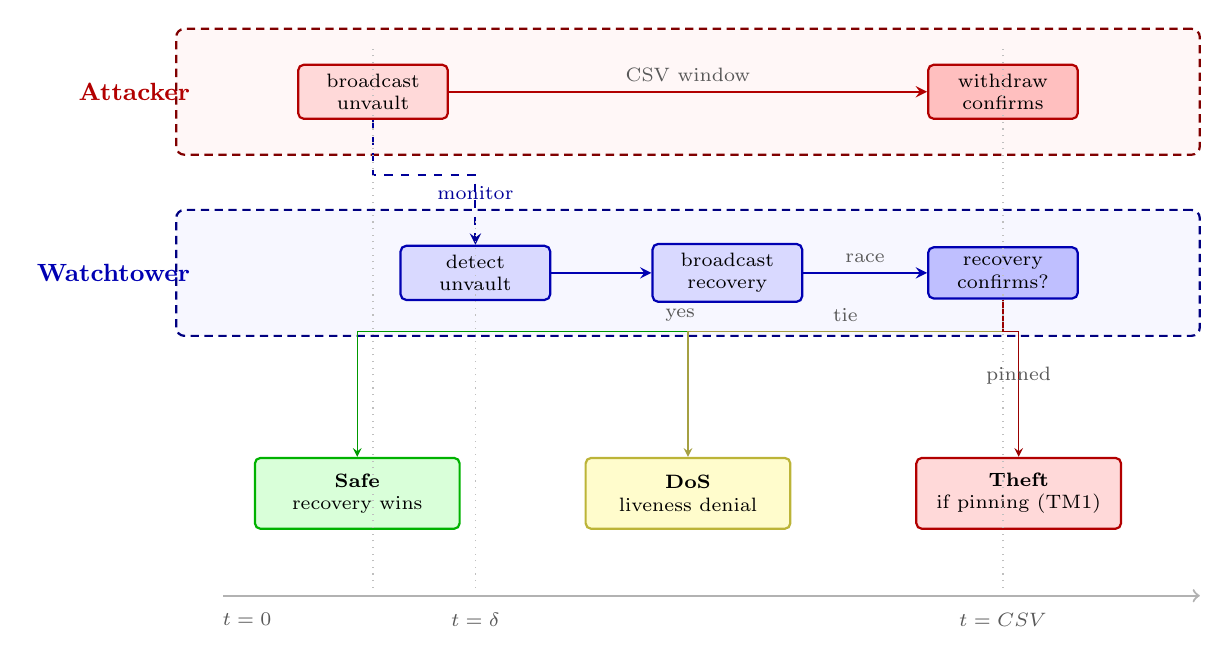
\begin{tikzpicture}[
  lane/.style={rectangle, draw, thick, minimum width=13cm, minimum height=1.6cm,
               rounded corners=3pt, dash pattern=on 3pt off 2pt},
  action/.style={rectangle, draw, rounded corners=2pt, minimum width=1.9cm,
                 minimum height=0.65cm, align=center, font=\scriptsize, thick},
  actatk/.style={action, fill=red!15, draw=red!70!black},
  actdef/.style={action, fill=blue!15, draw=blue!70!black},
  outcome/.style={rectangle, draw, rounded corners=2pt, minimum width=2.6cm,
                  minimum height=0.9cm, align=center, font=\scriptsize, thick},
  note/.style={font=\scriptsize, align=center, text=gray!70!black},
  tlabel/.style={font=\scriptsize, text=gray!70!black, anchor=north},
  edge/.style={draw, ->, >=stealth, thick},
]
  % ===== Attacker lane =====
  \node[lane, fill=red!3, draw=red!50!black] (alane) at (6.5, 3.0) {};
  \node[font=\small\bfseries, text=red!70!black, anchor=east] at (0.3, 3.0) {Attacker};

  \node[actatk] (au) at (2.5, 3.0) {broadcast\\ unvault};
  \node[actatk, fill=red!25] (aw) at (10.5, 3.0) {withdraw\\ confirms};
  \draw[edge, red!70!black] (au.east) -- (aw.west)
        node[midway, above, note] {CSV window};

  % ===== Watchtower lane =====
  \node[lane, fill=blue!3, draw=blue!50!black] (wlane) at (6.5, 0.7) {};
  \node[font=\small\bfseries, text=blue!70!black, anchor=east] at (0.3, 0.7) {Watchtower};

  \node[actdef] (wd) at (3.8, 0.7) {detect\\ unvault};
  \node[actdef] (wb) at (7.0, 0.7) {broadcast\\ recovery};
  \node[actdef, fill=blue!25] (wc) at (10.5, 0.7) {recovery\\ confirms?};
  \draw[edge, blue!70!black] (wd.east) -- (wb.west);
  \draw[edge, blue!70!black] (wb.east) -- (wc.west)
        node[midway, above, note] {race};

  % Monitor arrow (attacker -> watchtower) — routed to avoid overlap
  \draw[edge, dashed, blue!60!black] (au.south) -- ++(0, -0.7) -| (wd.north)
        node[pos=0.75, above, note, text=blue!60!black] {monitor};

  % ===== Outcomes row (below watchtower) =====
  \node[outcome, fill=green!15, draw=green!70!black] (safe) at (2.3, -2.1)
       {\textbf{Safe}\\ recovery wins};
  \node[outcome, fill=yellow!20, draw=yellow!70!black] (dos) at (6.5, -2.1)
       {\textbf{DoS}\\ liveness denial};
  \node[outcome, fill=red!15, draw=red!70!black] (theft) at (10.7, -2.1)
       {\textbf{Theft}\\ if pinning (TM1)};

  % Connect "recovery confirms?" to outcomes — fan-out with labels
  \draw[edge, thin, green!60!black] (wc.south) -- ++(0, -0.4) -| (safe.north)
        node[pos=0.25, above, note] {yes};
  \draw[edge, thin, yellow!60!black] (wc.south) -- ++(0, -0.4) -| (dos.north)
        node[pos=0.25, above, note] {tie};
  \draw[edge, thin, red!60!black] (wc.south) -- ++(0, -0.4) -| (theft.north)
        node[pos=0.75, above, note] {pinned};

  % ===== Timeline axis =====
  \draw[->, thick, gray!60] (0.6, -3.4) -- (13.0, -3.4);
  \node[tlabel] at (0.9, -3.5) {$t = 0$};
  \node[tlabel] at (3.8, -3.5) {$t = \delta$};
  \node[tlabel] at (10.5, -3.5) {$t = \text{CSV}$};

  % Vertical event guides (subtle)
  \draw[dotted, gray!50] (2.5, -3.3) -- (2.5, 3.55);
  \draw[dotted, gray!50] (3.8, -3.3) -- (3.8, 1.4);
  \draw[dotted, gray!50] (10.5, -3.3) -- (10.5, 3.55);

\end{tikzpicture}}
\caption{Trigger key theft race (\textbf{TM3}). The attacker broadcasts an
unvault (upper lane). The watchtower detects it at time $\delta$ and broadcasts
recovery (lower lane). The outcome hinges on whether recovery confirms before
CSV expiry: safe if recovery wins, DoS if tied, theft if the attacker successfully
pins the watchtower's transaction (combining TM3 with TM1).}
\label{fig:trigger_theft}
\end{figure}

\paragraph{CTV.} The hot key can trigger the unvault transaction and, after the CSV
delay, complete the withdrawal to the pre-committed destination. If the attacker also
holds the fee key (enabling fee pinning to block recovery), this escalates to fund
theft. Hot key alone produces liveness denial only---the defender sweeps to cold
storage.

\paragraph{CCV.} The trigger key can direct the withdrawal to an attacker-controlled
address (the destination is chosen at trigger time, not fixed at creation). The
watchtower races to invoke keyless recovery (122\vB{}). Since recovery is
permissionless, the watchtower needs no additional key material to respond.

\paragraph{OP\_VAULT.} The trigger key can redirect withdrawals, similar to CCV. The
watchtower races to invoke authorized recovery (246\vB{}), which requires the
\texttt{recoveryauth} key. If the attacker compromises both the trigger key and the
recoveryauth key, the result is persistent liveness denial (not theft), because the
recovery address is pre-committed in the vault's Taproot internal key tweak and cannot
be changed.

\paragraph{CAT+CSFS.} The hot key can only trigger to the pre-committed vault-loop
output. The dual CSFS+CHECKSIG verification binds the output to the embedded
\texttt{sha\_single\_output} constant---changing the output changes the sighash,
invalidating the signature. The hot key holder is limited to griefing (triggering
unwanted unvaults that the defender can recover from). This is the strongest hot-key
theft resistance of any design studied.

% ======================================================================
\section{Class \classcold{}: Cold-Key Theft via Unconstrained Recovery (TM11)} \label{se:cold_key_recovery}

Cold key compromise has asymmetric consequences depending on whether the recovery
path constrains outputs.

\begin{figure}[t]
\centering
\resizebox{0.95\textwidth}{!}{%
\begin{tikzpicture}[
  node distance=0.8cm,
  scenario/.style={rectangle, draw, rounded corners=3pt, thick,
                   minimum width=6.5cm, minimum height=5.8cm},
  hot/.style={scenario, fill=green!3, draw=green!60!black},
  cold/.style={scenario, fill=red!3, draw=red!60!black},
  leaf/.style={rectangle, draw, rounded corners=1pt, align=center,
               font=\scriptsize\ttfamily, minimum width=4.0cm,
               minimum height=0.7cm, fill=yellow!15, draw=yellow!60!black},
  op/.style={rectangle, draw, rounded corners=2pt, align=center,
             font=\scriptsize, minimum width=3.6cm, minimum height=0.6cm,
             fill=purple!10, draw=purple!60!black},
  bad/.style={rectangle, draw, rounded corners=2pt, align=center, thick,
              font=\scriptsize, minimum width=3.6cm, minimum height=0.6cm,
              fill=red!15, draw=red!70!black},
  good/.style={rectangle, draw, rounded corners=2pt, align=center, thick,
               font=\scriptsize, minimum width=3.6cm, minimum height=0.6cm,
               fill=green!15, draw=green!70!black},
  outcome/.style={rectangle, draw, rounded corners=2pt, align=center,
                  font=\scriptsize\bfseries, minimum width=4.0cm,
                  minimum height=0.9cm, thick},
  note/.style={font=\scriptsize, align=center, text=gray!70!black},
  edge/.style={draw, ->, >=stealth, thick},
]
  % LEFT SCENARIO: hot key compromise (safe)
  \node[hot] (hotbox) at (-4, 0) {};
  \node[font=\small\bfseries, text=green!60!black, above=-0.2cm of hotbox.north]
       {Hot key compromise (TM3)};
  \node[leaf] at (-4, 1.8) (hleaf) {hot leaf: CSFS + CHECKSIG};
  \node[op, below=0.3cm of hleaf] (csfs1) {OP\_CSFS(\,sig, hot\_pk,\\
        \scriptsize preimage\,)};
  \node[op, below=0.2cm of csfs1] (csig1) {OP\_CHECKSIG(\,sig, hot\_pk\,)};
  \node[good, below=0.3cm of csig1] (bind)
       {output bound by\\ \texttt{hashOutputs} in preimage};
  \node[outcome, below=0.3cm of bind, fill=green!20, draw=green!70!black]
       (safe) {SAFE\\ (griefing only)};

  % RIGHT SCENARIO: cold key compromise (total theft)
  \node[cold] (coldbox) at (4, 0) {};
  \node[font=\small\bfseries, text=red!70!black, above=-0.2cm of coldbox.north]
       {Cold key compromise (TM11)};
  \node[leaf, fill=red!10] at (4, 1.8) (cleaf) {recover leaf: cold\_pk OP\_CHECKSIG};
  \node[op, below=0.3cm of cleaf, fill=gray!15, draw=gray!60!black]
       (none) {\textit{no introspection}\\
              \scriptsize (\,no CAT, no CSFS\,)};
  \node[op, below=0.2cm of none, fill=gray!15, draw=gray!60!black]
       (nobind) {\textit{no output binding}\\ \scriptsize
                 SIGHASH\_DEFAULT allows any tx};
  \node[bad, below=0.3cm of nobind]
       (sweep) {attacker chooses\\ destination address};
  \node[outcome, below=0.3cm of sweep, fill=red!25, draw=red!80!black]
       (theft) {\textbf{TOTAL THEFT}\\ (125 vB, instant)};

  % Edges inside each box
  \draw[edge, green!60!black] (hleaf) -- (csfs1);
  \draw[edge, green!60!black] (csfs1) -- (csig1);
  \draw[edge, green!60!black] (csig1) -- (bind);
  \draw[edge, green!60!black] (bind) -- (safe);

  \draw[edge, red!60!black] (cleaf) -- (none);
  \draw[edge, red!60!black] (none) -- (nobind);
  \draw[edge, red!60!black] (nobind) -- (sweep);
  \draw[edge, red!60!black] (sweep) -- (theft);

  % Central contrast annotation
  \node[align=center, font=\scriptsize\itshape, text width=2.5cm]
       at (0, -0.3) {hot leaf:\\ output bound\\ \textbf{vs.}\\
                     cold leaf:\\ unconstrained};

\end{tikzpicture}}
\caption{CAT+CSFS asymmetric key safety. \textbf{Left:} hot key compromise leaks
only the trigger authority---the dual CSFS$\,+\,$CHECKSIG binding forces outputs
to match the embedded \texttt{sha\_single\_output} constant (\textbf{TM3} reduces
to griefing). \textbf{Right:} cold key compromise yields total theft (\textbf{TM11}):
the recovery leaf is bare \texttt{OP\_CHECKSIG}---no timelock, no introspection,
no destination constraint. The attacker sweeps funds to any address in one 125\vB{}
transaction.}
\label{fig:cold_key_theft}
\end{figure}

\paragraph{CAT+CSFS.} The recovery leaf is \texttt{cold\_pk
OP\_CHECKSIG} with \sighash{DEFAULT}: no introspection, no
timelock, no output constraint. Cold key compromise grants
immediate, unrestricted theft---the attacker sends all funds to an
arbitrary address in a 125\vB{} transaction indistinguishable from
legitimate recovery on-chain. Of the four designs, this is the
worst-case TM11 profile.

\paragraph{CTV.} The cold sweep is CTV-committed, sending funds to the pre-committed
cold address. Cold key compromise allows forced recovery but only to that address.
The attacker cannot redirect funds.

\paragraph{OP\_VAULT.} Recovery is output-constrained to the pre-committed recovery
address (embedded in the Taproot internal key tweak). Cold key compromise plus
recoveryauth key compromise yields persistent denial of service but not theft.

\paragraph{CCV.} Recovery is keyless and output-constrained. There is no cold key to
compromise in the recovery path.

\paragraph{Simplicity.} Both trigger and recovery enforce
\texttt{jet::outputs\_hash()}, constraining recovery to the pre-committed address.
Cold key compromise forces recovery but cannot redirect funds---matching CCV and
OP\_VAULT's output-constrained model.

The recovery safety ranking is: CCV (keyless, constrained) $>$ OP\_VAULT
(key-gated, constrained) $>$ CTV (key-gated, constrained) $>$ CAT+CSFS
(key-gated, \emph{unconstrained}). Poelstra~\cite{Poe21} proposed an alternative
CAT+CSFS recovery design using recursive staging resets, where cold key compromise
leads to a liveness battle rather than immediate theft. Under that design, the
attacker and owner take turns resetting the vault state, each paying transaction fees
per round. This would upgrade CAT+CSFS's recovery safety to match OP\_VAULT's
(liveness denial, not theft), but at the cost of a larger recovery script and
additional witness overhead.

% ======================================================================
\section{Projection onto the $(g, b)$ Sublattice} \label{se:two_dim}

The design-space decomposition of Section~\ref{ss:design_space} induces
a natural projection onto the $(g, b)$ sublattice---the two recovery-path
dimensions---whose structure captures the recovery-related tradeoffs
without appeal to per-design measurement.

\begin{lemma}\label{lem:projection}
Let $D = (f, a, g, b)$ be a design with uniform leaf binding (hot and
cold paths share the same~$b$). Then:
\begin{enumerate}
  \item As $g$ weakens from $g_{\text{key}}$ to $g_{\text{keyless}}$,
    $\mathcal{L}(\mathrm{TM2})$ increases by
    Lemma~\ref{lem:keyless_grief}, while the key-loss attack surface
    vanishes.
  \item As $b$ weakens from $b_{\text{bound}}$ to $b_{\text{unbound}}$,
    $\mathcal{L}(\mathrm{TM11})$ increases from $0$ to $V$ by
    Lemma~\ref{lem:unbound_theft}.
  \item The cell $(g_{\text{keyless}}, b_{\text{unbound}})$ is
    unreachable: under Proposition~\ref{thm:griefing_safety}, a
    keyless vault with unbound recovery admits any party to invoke
    recovery to any destination, which is vacuous as a custody
    construction. No proposed BIP occupies this cell.
\end{enumerate}
\end{lemma}

\begin{proof}
Parts~1 and~2 are direct reinstatements of
Lemmas~\ref{lem:keyless_grief} and~\ref{lem:unbound_theft} with the $g$
and $b$ axes read individually. Part~3: if $\mathcal{A}(\emptyset) = 1$
and the recovery output is attacker-chooseable, any third party can
sweep the vault to their own address, reducing the construction to a
fee-free taproot \texttt{OP\_CHECKSIG} on a keyed path with no custody
benefit. \qed
\end{proof}

\begin{remark}\label{rem:asymmetric_binding}
Designs with \emph{asymmetric} leaf binding---hot leaf output-bound
and cold leaf unbound, as in CAT+CSFS---occupy two distinct cells in
this projection, one per leaf. The hot leaf sits at
$(g_{\text{key}}, b_{\text{bound}})$; the cold leaf sits at
$(g_{\text{key}}, b_{\text{unbound}})$. The ``off-axis'' position of
CAT+CSFS in a naive scatter visualisation is a direct consequence of
this leaf-level asymmetry, not an anomaly requiring a separate axis.
\end{remark}

\begin{figure}[t]
\centering
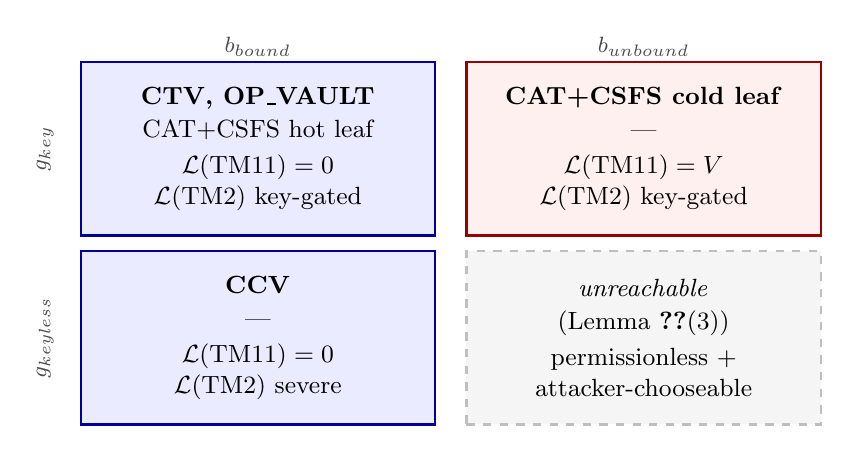
\begin{tikzpicture}[
  cell/.style={rectangle, draw, thick, minimum width=4.5cm,
               minimum height=2.2cm, align=center, font=\small},
  filled/.style={cell, fill=blue!8, draw=blue!60!black},
  asym/.style={cell, fill=red!6, draw=red!60!black},
  empty/.style={cell, fill=gray!8, draw=gray!50, dashed},
  axlbl/.style={font=\footnotesize\bfseries, text=gray!60!black,
                align=center},
]
  \node[axlbl] at (-0.5, 3.3) {$b_{\text{bound}}$};
  \node[axlbl] at (4.4, 3.3) {$b_{\text{unbound}}$};
  \node[axlbl, rotate=90] at (-3.2, 2.0) {$g_{\text{key}}$};
  \node[axlbl, rotate=90] at (-3.2, -0.4) {$g_{\text{keyless}}$};

  \node[filled] at (-0.5, 2.0) {\textbf{CTV, OP\_VAULT}\\[1pt]
        CAT+CSFS hot leaf\\[2pt]
        $\mathcal{L}(\mathrm{TM11})=0$\\
        $\mathcal{L}(\mathrm{TM2})$ key-gated};
  \node[asym] at (4.4, 2.0) {\textbf{CAT+CSFS cold leaf}\\[1pt]
        ---\\[2pt]
        $\mathcal{L}(\mathrm{TM11})=V$\\
        $\mathcal{L}(\mathrm{TM2})$ key-gated};
  \node[filled] at (-0.5, -0.4) {\textbf{CCV}\\[1pt]
        ---\\[2pt]
        $\mathcal{L}(\mathrm{TM11})=0$\\
        $\mathcal{L}(\mathrm{TM2})$ severe};
  \node[empty] at (4.4, -0.4) {\emph{unreachable}\\[1pt]
        (Lemma~\ref{lem:projection}(3))\\[2pt]
        permissionless +\\
        attacker-chooseable};
\end{tikzpicture}
\caption{Projection of the covenant design space onto the $(g, b)$
sublattice. Three cells are occupied by the four proposed Bitcoin
Script extensions; the fourth is structurally unreachable. CAT+CSFS
appears in two cells by Remark~\ref{rem:asymmetric_binding}.}
\label{fig:two_dim}
\end{figure}

A practitioner choosing between designs must evaluate both dimensions relative to
their threat model. An exchange prioritizing hot-key theft resistance (the most
likely attack vector for an online system) would favor CAT+CSFS, accepting the
cold-key risk and mitigating it through hardware security modules. A custodian
prioritizing recovery flexibility (e.g., an estate planning trust that must recover
under uncertain key availability) would favor CCV's keyless recovery, accepting the
griefing surface.

% ======================================================================
\section{Threat Model Matrix} \label{se:tm_matrix}

Table~\ref{tab:tm_full} presents the complete threat model matrix across all
eleven attack classes and four Bitcoin covenant designs. Each cell summarizes the
attack's severity and the measured vsize cost. The Simplicity mapping is omitted
from the matrix because it runs on a federated sidechain with fundamentally
different trust assumptions (Section~\ref{se:simplicity_bg}); its per-TM mapping
appears in Section~\ref{se:simplicity_measurements}.

\begin{table}[p]
\centering
\caption{Threat model matrix (TM1--TM11). Severity labels are bolded
uniformly; every ``N/A'' cell carries a one-phrase reason. Severity
scale: \textbf{N/A} = structurally impossible; \textbf{Low} = requires
difficult preconditions; \textbf{Moderate} = feasible under specific
conditions; \textbf{High} / \textbf{Severe} = significant risk under
realistic assumptions; \textbf{Safe} = correct behaviour by design.}
\label{tab:tm_full}
\footnotesize
\begin{tabular}{@{}cp{2.6cm}p{2.6cm}p{2.6cm}p{2.6cm}@{}}
\toprule
TM & CTV & CCV & OP\_VAULT & CAT+CSFS \\
\midrule
1 & \textbf{High.} 25-desc chain blocks CPFP (14{,}300 sats).
  & \textbf{N/A} (no anchor).
  & \textbf{N/A} (fee wallet).
  & \textbf{N/A} (external fee input). \\[6pt]

2 & \textbf{Moderate.} Hot key triggers; defender sweeps cold (133\vB).
  & \textbf{Severe.} Keyless, $\gamma{=}0.27$.
  & \textbf{Low.} Auth key needed, $\gamma{=}0.55$.
  & \textbf{Low.} Cold key needed; moot if TM11. \\[6pt]

3 & \textbf{High.} Hot+fee = theft; hot alone = DoS.
  & \textbf{High.} Redirect withdrawal; watchtower races (122\vB).
  & \textbf{Moderate.} Redirect; authorised recovery races (246\vB).
  & \textbf{Low.} Grief only (dual verification). \\[6pt]

4 & \textbf{N/A} (no revault).
  & \textbf{Severe.} 6{,}172 splits/block.
  & \textbf{Severe.} 3{,}427 splits/block.
  & \textbf{N/A} (no revault). \\[6pt]

5 & \textbf{N/A} (no xpub derivation).
  & \textbf{N/A} (no xpub derivation).
  & \textbf{Moderate.} xpub expansion leaks children.
  & \textbf{N/A} (no xpub derivation). \\[6pt]

6 & \textbf{High.} Hot+fee = theft.
  & \textbf{N/A} (single key).
  & \textbf{High.} Trigger+auth = persistent DoS.
  & \textbf{High.} Cold key alone = theft (TM11). \\[6pt]

7 & \textbf{High.} Stuck funds on address reuse.
  & \textbf{Safe.}
  & \textbf{Safe.}
  & \textbf{Safe.} \\[6pt]

8 & \textbf{N/A} (no mode byte in CTV).
  & \textbf{Developer footgun.} Undefined mode $\rightarrow$ \texttt{OP\_SUCCESS}.
  & \textbf{N/A} (no mode byte in \opvault{}).
  & \textbf{N/A} (no mode byte in CAT+CSFS). \\[6pt]

9 & \textbf{N/A} (no CSFS path).
  & \textbf{N/A} (no CSFS path).
  & \textbf{N/A} (no CSFS path).
  & \textbf{Impossible.} Dual verification. \\[6pt]

10 & \textbf{N/A} (no CSFS witness to manipulate).
   & \textbf{N/A} (no CSFS witness to manipulate).
   & \textbf{N/A} (no CSFS witness to manipulate).
   & \textbf{Impossible.} SHA-256 binding. \\[6pt]

11 & \textbf{N/A} (CTV-committed recovery).
   & \textbf{N/A} (keyless recovery; no cold key).
   & \textbf{N/A} (Taproot-tweak-constrained recovery).
   & \textbf{High.} Unconstrained CHECKSIG = immediate theft. \\
\bottomrule
\end{tabular}
\end{table}

% ======================================================================
\section{Deployment Guidance} \label{se:deployment}

Proposition~\ref{thm:fee_inversion} and the per-threat analysis yield fee-conditional
deployment recommendations:

\begin{itemize}
\item \textbf{Low-fee environments} ($r < 10$~sat/vB). Watchtower exhaustion is
  economically infeasible (too many splits needed, each recovery cheap). Fee pinning
  is cheap but CTV's exposure is small relative to vault value. CCV or OP\_VAULT are
  preferred because their additional capabilities (partial withdrawal, batching) come
  at negligible security cost.

\item \textbf{High-fee environments} ($r > 100$~sat/vB). Watchtower exhaustion
  becomes viable against CCV and OP\_VAULT---the watchtower's recovery budget scales
  linearly with fee rate, and dust-sized UTXOs become unrecoverable faster. CTV's
  fee pinning cost remains negligible. CTV is preferred in high-fee environments for
  vaults that do not require partial withdrawal or batching.

\item \textbf{Mixed or uncertain fee environments.} OP\_VAULT offers the best
  compromise: it has the strongest griefing resistance (authorized recovery), supports
  partial withdrawal and batching, and its per-UTXO recovery-cost scaling exposure is partially
  mitigated by the higher per-split cost that slows the attacker. However, BIP-345 has
  been withdrawn; the closest active proposal with similar properties is CCV (BIP-443)
  with application-level recovery authorization.

\item \textbf{Hot-key theft priority.} If the primary threat is hot-key compromise
  (e.g., an exchange or online service), CAT+CSFS provides the strongest resistance:
  the dual verification binding limits a hot-key attacker to griefing, with no path to
  fund redirection. The tradeoff is the cold-key vulnerability (TM11), which must be
  mitigated through operational security (hardware security modules, geographic
  distribution, multisig).
\end{itemize}

% ======================================================================
\section{Class \classmode{}: Mode/Parameter Bypass (TM8)}
\label{se:class_mode_bypass}

Class \classmode{} is enabled by axis \axopsurf{} =
\texttt{multi-mode-with-OP\_SUCCESS}: a polymorphic covenant opcode
takes a stack-provided mode selector, and the taproot
\texttt{OP\_SUCCESSx} upgrade mechanism promotes undefined mode
values to unconditional script success. A developer or construction
bug that selects an undefined mode silently disables the covenant
check.

\subsection{Susceptibility}
CCV is susceptible and is the only proposal with \axopsurf{} =
\texttt{multi-mode-with-OP\_SUCCESS}. BIP-443 defines four valid
modes $\{-1, 0, 1, 2\}$; any other value falls through to
\texttt{OP\_SUCCESSx}, which under BIP-341/BIP-342 taproot rules
terminates script execution with success regardless of stack state.
Five undefined modes $\{3, 4, 7, 128, 255\}$ were measured on
regtest; each produces full covenant bypass at $110\vB{}$ per spend.
$\mathcal{L}(\mathrm{TM8}) = V$.

\subsection{Immunity Derivations}
CTV, OP\_VAULT, and CAT+CSFS have \axopsurf{} = \texttt{single-mode}:
each exposes a single semantic opcode with no mode selector, so the
\texttt{OP\_SUCCESSx} fallthrough surface does not arise.

\subsection{Framing: Specified Behaviour, Not a Novel Vulnerability}
The class is \emph{specified behaviour} under BIP-443's
forward-compatibility design (itself inherited from BIP-341/BIP-342),
not a newly-discovered vulnerability. The contribution here is the
systematic mode sweep and the class-level framing that ties the
surface to axis \axopsurf{}, not the discovery of
\texttt{OP\_SUCCESSx} semantics. In practice, the pymatt reference
library mitigates the risk by providing named constants
(\texttt{CCV\_FLAG\_*}); the residual risk is in independent
implementations that hand-write the mode byte. We include this class
in the security analysis because the framework predicts the
vulnerability surface from axis position; omitting it would leave
axis \axopsurf{} under-motivated.

\subsection{Rationality and Scope}
\label{ss:rat_classmode}
\begin{description}
\item[(1) Attacker capability.] Any observer of a vault whose script
  contains an undefined mode byte; no keys required.
\item[(2) Defender model.] Developer discipline around mode-byte
  selection; library-provided named constants; code review.
\item[(3) Economic preconditions.] None applicable ---
  full vault bypass at constant $110\vB{}$/spend.
\item[(4) Protocol / network assumptions.] BIP-341/BIP-342
  \texttt{OP\_SUCCESSx} taproot upgrade semantics.
\item[(5) Scope of validity.] Applies iff \axopsurf{} =
  \texttt{multi-mode-with-OP\_SUCCESS}. The other three
  Bitcoin proposals are immune by construction.
\item[(6) Rational-attacker check.] Rational whenever a misconfigured
  vault exists on-chain; the attacker's payoff is $V$, the cost is
  a single spend of $110\vB{} \times r$.
\item[(7) Counter-factual mitigations.] (a) \axopsurf{} =
  \texttt{single-mode} (one opcode per primitive, as in the other
  three proposals); (b) bitmask-gated mode check at script-parse
  time (reject undefined modes before execution) --- would eliminate
  the class without revising soft-fork semantics but would forfeit
  the forward-compatibility benefit; (c) pymatt-style named
  constants (\texttt{CCV\_FLAG\_*}) that make the undefined-mode
  surface unreachable from application code.
\end{description}

% ======================================================================
\section{Rationality Blocks for Classes Z1--Z5}
\label{se:rationality_blocks}

Each of the attack classes analysed in
Sections~\ref{se:fee_pinning}--\ref{se:cold_key_recovery} admits a
seven-field \emph{Rationality and Scope} block per the schema of
Section~\ref{se:rationality_conventions}. We compress the blocks
below; Appendix~D carries the uncompressed free-text form. Each
field implicitly cites the Kerckhoffs threat model of
Section~\ref{ss:kerckhoffs}.

\subsection{Class \classfee{} (Fee-Channel Pinning)}
\label{ss:rat_classfee}
\begin{description}[leftmargin=1.5em,itemsep=1pt,parsep=0pt]
\item[(1) Attacker capability.] Hot key; capital for the
  anchor-descendant chain ($\approx 14{,}300$~sats at
  $\rho = 3\satvB{}$).
\item[(2) Defender model.] Online watchtower; Bitcoin Core default
  mempool policy with $25$-descendant limit (BIP-125).
\item[(3) Economic preconditions.] $\mathcal{L}$ and
  $\mathrm{Adv}$ are $r$-invariant; rational at any fee regime.
\item[(4) Protocol / network assumptions.] BIP-125 Rule 3 requires
  the watchtower's CPFP replacement to pay for evicting every
  descendant; $3\satvB{}$ Core default dustRelay is policy not
  consensus.
\item[(5) Scope of validity.] Applies iff \axfee{} =
  \texttt{out-of-band-anchor}. N/A for dynamic fee models (CCV, OPV,
  CAT+CSFS).
\item[(6) Rational-attacker check.] Rational at any $r$ given hot key;
  yield $\approx V$ at marginal cost.
\item[(7) Counter-factual mitigations.] (a) TRUC/BIP-431 collapses
  the descendant limit to $1$, eliminating the class at the
  relay-policy level; (b) cluster-mempool redesign qualitatively
  changes the replacement calculus (scope-limit); (c) P2A-style
  smaller anchor output reduces the absolute cost of the attack but
  does not eliminate the structural surface.
\end{description}

\subsection{Class \classgrief{} (Permissionless Griefing)}
\label{ss:rat_classgrief}
\begin{description}[leftmargin=1.5em,itemsep=1pt,parsep=0pt]
\item[(1) Attacker capability.] Zero keys (for CCV). Observation of
  mempool plus the public recovery address.
\item[(2) Defender model.] Any; the attack is pure liveness denial
  and ends only when the defender abandons or rotates the vault.
\item[(3) Economic preconditions.] $\mathcal{L}$ scales linearly in
  $r$; $\gamma = \text{vsize}_{\text{atk}}/\text{vsize}_{\text{def}}$
  is $r$-invariant.
\item[(4) Protocol / network assumptions.] Mempool-observable trigger
  tx; no RBF dependence.
\item[(5) Scope of validity.] Applies iff \axauth{} =
  \texttt{keyless}. Reduces to a key-compromise attack (TM6)
  otherwise.
\item[(6) Rational-attacker check.] Irrational without external
  incentive (no financial gain). Rational only under extortion,
  competitor disruption, or state-actor threat.
\item[(7) Counter-factual mitigations.] \axauth{} =
  \texttt{recoveryauth-key} (as in OP\_VAULT) or key-gated recovery
  (CTV, CAT+CSFS) eliminates the class by forcing a signature on
  the recovery leaf.
\end{description}

\subsection{Class \classscale{} (Per-UTXO Recovery-Cost Scaling)}
\label{ss:rat_classscale}
\begin{description}[leftmargin=1.5em,itemsep=1pt,parsep=0pt]
\item[(1) Attacker capability.] Trigger key; capital for $N$ partial
  unvaults.
\item[(2) Defender model.] Watchtower with recovery authority;
  batching flag $b$; minimal-disruption policy (reactive per-UTXO
  recovery) maximises attacker leverage. A full-sweep-on-first-alert
  policy collapses the class to one round at the cost of operational
  disruption.
\item[(3) Economic preconditions.] Rate-dependent; threshold
  $r^\dagger_{\mathrm{TM4}}$ per Equation~\ref{eq:r_star}. Below
  the threshold the defender can absorb the per-UTXO liability
  before dust economics kick in.
\item[(4) Protocol / network assumptions.] Bitcoin dust thresholds
  ($546$~sats P2WPKH, $330$~sats P2TR). RBF rule 3 does not permit
  sibling-eviction, so the attacker's partial-withdrawal chain is
  single-chain. Minimum relay fee $\approx 1\satvB{}$.
\item[(5) Scope of validity.] Applies iff \axrevault{} =
  \texttt{yes}. The class is a structural cost tail of partial
  withdrawal, independent of adversary behaviour; an attacker
  accelerates the distribution but is not required.
\item[(6) Rational-attacker check.] Rational only above $r^\dagger$
  with external incentive (competitor, extortion). Pure liveness
  attacker is irrational at any $r$ (no gain). Attacker with hot
  key can extract value from abandoned UTXOs post-CSV.
\item[(7) Counter-factual mitigations.] (a) Defender batching raises
  $r^\dagger$ by $1.8$--$2.7\times$; (b) full-sweep-on-first-alert
  collapses the loop; (c) operational limits on per-epoch trigger
  count.
\end{description}

\paragraph{Reframing note.}
Earlier framings of this class as ``watchtower exhaustion'' cast it
as a multi-round attacker-vs-watchtower game. That framing does not
survive a defender with full recovery authority who can full-sweep
on first alert, collapsing the multi-round narrative to one round.
The reframe above identifies the class as a structural cost tail of
partial withdrawal --- attacker-accelerable but not
attacker-required --- with the defender's degree of freedom in
recovery batching. The multi-round attacker scenario remains one
\emph{threat-model instantiation} among several, documented in
Appendix~D.

\subsection{Class \classhot{} (Hot-Key Theft via Destination Substitution)}
\label{ss:rat_classhot}
\begin{description}[leftmargin=1.5em,itemsep=1pt,parsep=0pt]
\item[(1) Attacker capability.] Hot key; mempool access; optional
  fee-pinning capital (if class \classfee{} composes).
\item[(2) Defender model.] Online watchtower able to race during the
  CSV delay; race bias toward attacker under class-\classfee{}
  composition (CTV).
\item[(3) Economic preconditions.] Race outcome $r$-independent
  except via class \classfee{}.
\item[(4) Protocol / network assumptions.] CSV delay length; mempool
  propagation dynamics (Riard's cycling attack is out of scope).
\item[(5) Scope of validity.] Applies iff \axwdbind{} $\neq$
  \texttt{signature-dual-bind}.
\item[(6) Rational-attacker check.] Rational only paired with
  fee-pinning budget (composition with class \classfee{}); otherwise
  the defender wins the race generically.
\item[(7) Counter-factual mitigations.] \axwdbind{} =
  \texttt{signature-dual-bind} (CAT+CSFS) eliminates the class by
  cryptographic construction: the Schnorr EUF-CMA reduction forces
  the assembled preimage to equal the consensus preimage, binding
  \texttt{hashOutputs} and foreclosing destination substitution.
\end{description}

\subsection{Class \classcold{} (Cold-Key Theft via Unconstrained Recovery)}
\label{ss:rat_classcold}
\begin{description}[leftmargin=1.5em,itemsep=1pt,parsep=0pt]
\item[(1) Attacker capability.] Cold key (Kerckhoffs: the attack
  assumes compromise, not inference).
\item[(2) Defender model.] Any; the attack is instant with no CSV
  window, no watchtower intervention window.
\item[(3) Economic preconditions.] $r$-invariant.
\item[(4) Protocol / network assumptions.] N/A --- pure signature
  check; no mempool dynamics.
\item[(5) Scope of validity.] Applies iff \axrecbind{} =
  \texttt{plain-signature}.
\item[(6) Rational-attacker check.] Rational whenever cold key is
  compromised; yield $V$.
\item[(7) Counter-factual mitigations.] \axrecbind{} =
  \texttt{signature-dual-bind} on the recovery leaf (Poelstra's
  sketch for CAT+CSFS-based bound recovery) would move the design
  to an immune axis position, eliminating the class. Alternative
  \axrecbind{} values (\texttt{template-hash-digest},
  \texttt{per-output-amount+script}, \texttt{dedicated-opcode}) as
  in CTV, CCV, OPV also produce immunity.
\end{description}
